\section{Introduction}
\label{sec:intro}
Personalized dialogue systems are promising NLP applications for human-computer interaction and emotional companionship. We would expect such systems to have personalities (gender, age, hobbies, etc.), exhibit emotions, take dialogue acts and even adopt sophisticated strategies \citep{liu2021towards}, which necessitates the research efforts on \textit{Controllable Text Generation}. Specifically, the simultaneous controlling of \textit{multiple attributes} as discussed above is vital to handle the complexity of these chatbots, and can significantly ameliorate their expressiveness, human-likeness, and explainability. However, despite great recent progress in controllable text generation \citep{dathathri2019plug,keskar2019ctrl,krause2021gedi}, multi-attribute control is still under-explored. 
% \MY{Why is multi-attribute control important? Imply that affect, emotion, etc. are complexed and human-likeness indicates combinations of these}
% \textit{Controllable Text Generation} is the technique to steer the generated content with desired attribute(s). It has the potential to generate articles about specific topics \citep{keskar2019ctrl}, help reduce the toxicity of the generation \citep{gehman2020realtoxicityprompts} and alleviate repetitiveness and dullness \citep{arora2022director}. It can be especially promising for building personalized dialogue systems, which should .

In this paper, we explore a novel task of \textit{Multi-Attribute Controllable 
Dialogue Generation}. The numerous combinations of attributes can make the available data for each setting scarce, which poses a great challenge for this task. We thus resort to the paradigm of \textit{Weighted Decoding} as our starting point, which has achieved great success in previous single-attribute control tasks~\citep{arora2022director}. 
Weighted decoding methods learn a token-level attribute classifier, 
which predicts the probability of the text conveying the desired attribute 
given the generation of each token in the vocabulary. 
Then the predicted probabilities are used to 
re-weight the token generation during decoding to induce the attribute. 
Although these methods have shown strong controllability in single-attribute control, they will have issues when extended to the multi-attribute case 
by multiplying several attribute predictions from multiple classifiers. Extra 
parameters proportional to the large vocabulary size $|V|$ will be introduced, 
which can grow severalfold further according to the number of attributes. 
The consequent large number of parameters will not only make the model inefficient, but also harm the generation quality. The model can be prone to overfit since the data for each attribute combination are usually small, which increases the risk of degeneration \citep{holtzman2019curious}. 
% \MY{is small training data a definite condition? why do we need to care its degeneration on small data? if you'd like to discuss that for multi attribute learning, inevitable situation is small training data, you could elaborate a bit here}
% \MY{what do you mean by saying the original version? just Director? Here we did not mention that the current method is an evolved version}

\begin{figure}[th]
    \centering
    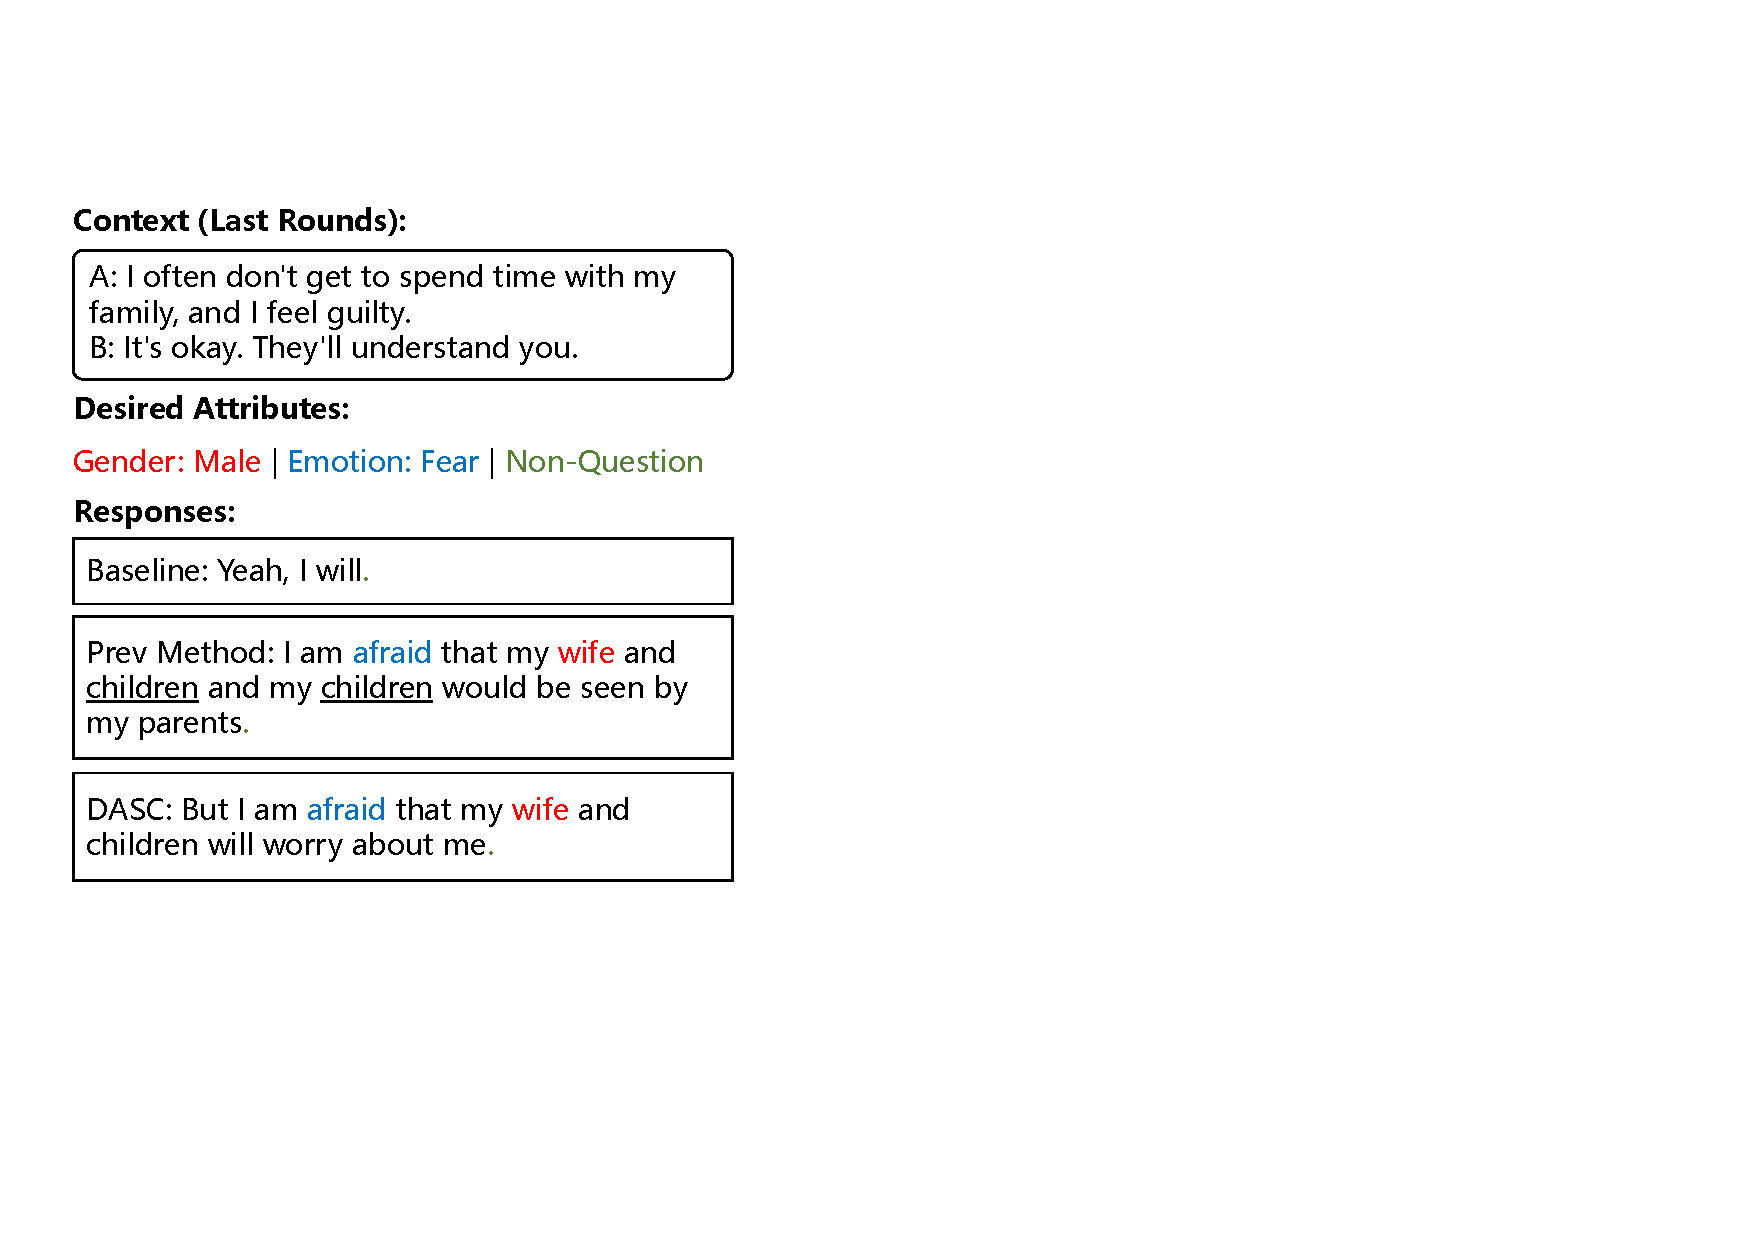
\includegraphics[width=1.0\columnwidth]{figures/teaser_example.pdf}
    \caption{An example of multi-attribute controllable dialogue generation. The baseline system doesn't leverage any control signal and produced a dull response, while the previous method for controlling generated repetitive and illogical text. DASC successfully gives a response both fluent and attributed.}
    \label{fig:teaser_example}
\end{figure}
% \KZ{In this example, the context already contains the words ``my wife'', so
% producing ``my wife'' in the response is not so surprising, and may not be
% taken as the result of applying gender attribute control. How about
% removing the ``my wife and'' in the context? If the response
% still contains my wife, then it makes a strong case. Also, instead of 
% controling the attributes to ``Non-question'', do a ``Question'' might be more
% interesting. Since this is a canonical example, it might not even be real.
% You can change the ``Baseline'' and ``M-Director'' to ``Previous method 1''
% and ``Previous method 2'', and DASC to ``Desired response.'' At this point in
% the text, u actually haven't talked about M-Director, so i think it's ok
% to just call them previous methods.}
% \ZL{Adjusted the example, Since questions usually don't contain interesting content, I don't show such example here.}

To overcome these limitations, we propose \textbf{D}ialog \textbf{A}ttribute \textbf{S}pace \textbf{C}ontroller (\textbf{DASC}). We establish an attribute semantic space where each token in the vocabulary is projected to the space through \textit{Attribute Token Embedding} shared across attributes. The language models' hidden states are also converted to \textit{Attribute Context Embedding} in the space through attribute-specific layers. We then assign higher weights for the neighboring tokens of the current context embedding in the attribute space during decoding, which is implemented with a dot-product-based attribute classifier.
Consequently, DASC can inherit the strong controllability of weighted decoding, while also achieving a natural solution of multi-attribute control with the interpolation of multiple attribute embeddings in the space. Moreover, the shared attribute token embedding also alleviates over-parameterization, and improves the robustness of the model.
% \MY{Are there any other previous methods on multiple attributes? We still lack talking about the pros of using such latent space, which is very important so should better put it earlier}
% \ZL{Not easy to compare across different families of such methods. I opt to focus on weighted decoding to make the argument clear. But I do added more emphases on our strength.}

We experiment on an attribute-rich open-domain dialogue dataset \citep{xu2022long} for the simultaneous control of 3 attribute aspects: Gender Style (male, female, neutral), Emotion (8 classes) ,and a simple division of Dialogue Act (question VS non-question). 
As exemplified in Figure \ref{fig:teaser_example}, 
compared to previous methods, DASC achieves strong controllability while 
avoiding low-quality generations in the compositional controlling task. 
Visualization of the attribute token embeddings exhibits specific patterns 
that benefit the controlling, compared to the general LM token embeddings. 
A robustness test that requires the models to generate responses 8 times 
with any single emotion further shows that the controllability of 
DASC can generalize in this out-of-distribution setting.  

Our contributions are as follows: 
\begin{enumerate}
    \item We propose semantic space grounded weighted decoding for controllable dialogue generation, which can intuitively solve the multi-attribute control task with the interpolation of embeddings in the space.
    \item Experiments show that the proposed method can achieve state-of-the-art accuracy on the simultaneous control of 3 aspects while also preserving competitive generation quality in both conventional test settings and out-of-distribution robustness tests.
    \item We also demonstrate more potential applications like blending two emotions or adopting emotional support strategies in the generated response.
\end{enumerate}

%\KZ{Perhaps we should tone-down a bit and not say SOTA since we only experimented on one dataset?}
%\ZL{I've also experimented on another Chinese dataset Diamante for emotion control, the advantage is even higher. I'm not presenting this dataset as it has overrided by the current DuLemon dataset (with more attributes and larger size). Experiments on the English ESConv dataset also supports DASC's advantage, and will be discussed.}
